\documentclass[a4paper,12pt]{article}
\usepackage[utf8]{inputenc}
\usepackage[T1]{fontenc}
\usepackage[czech,english]{babel}
\usepackage{graphicx}
\usepackage{hyperref}
\usepackage{geometry}
\usepackage{xcolor}
\usepackage{float}
\usepackage{mdframed}
\usepackage{amsmath}
\geometry{margin=2.5cm}

\setlength{\parskip}{0.8em}
\setlength{\parindent}{0pt}

\begin{document}
	
	\begin{center}
		{\Large \textbf{BPA-KOM Lab 4 -TCP and UDP}}\\[1em]
	\end{center}
	
	\vspace{1cm}
	
	\begin{center}
		\begin{tabular}{|c|c|}
			\hline
			\textbf{Name} & Dave Galea \\ \hline
			\textbf{VUT ID} & 284844 \\ \hline
			\textbf{Lab Number} & 4 \\ \hline
			\textbf{Date} & December 2025 \\ \hline
		\end{tabular}
	\end{center}
	
	\vspace{0.5cm}
	\hrule
	\vspace{0.5cm}
	
	\section*{1. Objective 1}
	
	\textbf{Task Assignment:} The aim of this task was to analyse UDP packets using the DNS protocol in Wireshark.
	
	\textbf{Solution:}\\[1em]
	After starting to capture packets in Wireshark, in CMD, the \texttt{nslookup} command was executed which takes the executer to the interactive mode. \texttt{type=A} was set to query only IPv4 addresses, and the IP address for the domain was set as \texttt{www.vut.cz}. The result of the above is the following:
	\begin{figure}[H]
		\centering
		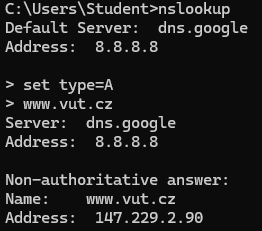
\includegraphics[width=\linewidth, height=0.2\textheight, keepaspectratio]{photos/1-4}
		\caption{Output of \texttt{nslookup}.}
	\end{figure}
	
	In Wireshark, the Filter was set to the following: \texttt{dns.qry.name==www.vut.cz.localdomain}. This displays only the DNS query-response that was issued. The output after setting the filter is the following:
	\begin{figure}[H]
		\centering
		
\includegraphics[width=\linewidth, height=0.4\textheight, keepaspectratio]{photos/1-5}
		\caption{Output in Wireshark after setting the stated filter.}
	\end{figure}
	
	Upon expanding the query message, it can be noted that UDP is used as the transport layer protocol. After expanding User Datagram Protocol section, the output is the following: 
	\begin{figure}[H]
		\centering
		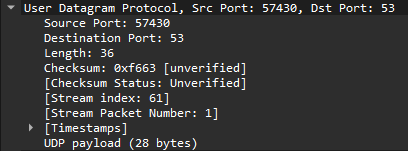
\includegraphics[width=\linewidth, height=0.3\textheight, keepaspectratio]{photos/1-6}
		\caption{Expansion of User Datagram Protocol section of query message}
	\end{figure}
	The output matches what is discussed in the introduction; the length is 36 bytes, while the payload (data) is 28bytes, meaning that the header is 8 bytes. This is because the header consists of 4 sections, each of 2 bytes each; the Source Port, the Destination port, the Length, and the Checksum. 
	
	Upon expanding the response message, the output is as following:
	\begin{figure}[H]
		\centering
		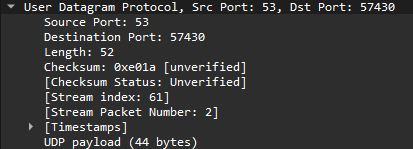
\includegraphics[width=\linewidth, height=0.3\textheight, keepaspectratio]{photos/1-7}
		\caption{Expansion of User Datagram Protocol section of response message}
	\end{figure}
	When comparing the expansion of the respective User Datagram Protocol sections of the query and response messages, it can be noted that the source and destination ports swap values. In both, the UDP header size still remains the same value of 8 bytes. 
	
	
	
	\vspace{1em}
	\hrule
	\vspace{0.5em}
	
	\section*{2. Objective 2}
	
	\textbf{Task Assignment:} The aim of this task was to analyse TCP packets using the DNS protocol in Wireshark.
	
	\textbf{Solution:}\\[1em]
	After typing \texttt{set vc} in CMD so to enforce DNS to establish virtual circuit and use TCP, the query for \texttt{www.vut.cz} was issued again. With the same filter as before still applied, it can be seen in the output below that 2 new records appear. 
	\begin{figure}[H]
		\centering
		
\includegraphics[width=\linewidth, height=0.4\textheight, keepaspectratio]{photos/2-3}
		\caption{Output in Wireshark after typing \texttt{set vc} in CMD.}
	\end{figure}
	
	Upon right clicking on one of the new messages, followed by \textbf{Follow > TCP Stream}, one can observe the captured TCP steam. 
	
	\begin{figure}[H]
		\centering
		
\includegraphics[width=\linewidth, height=0.4\textheight, keepaspectratio]{photos/2-4}
		\caption{Captured TCP steam using DNS.}
	\end{figure}
	
	The first 3 messages in the TCP stream were exchanged so to establish the virtual circuit. Upon examining the first message, the output is as follows:
	
	\begin{figure}[H]
		\centering
		
\includegraphics[width=\linewidth, height=0.4\textheight, keepaspectratio]{photos/2-6}
		\caption{First TCP message}
	\end{figure}
	
	The non optional parts of the TCP header include: Source port, Destination port, Sequence number, Acknowledgement number, Header length, and reserved. These together occupy 20 bytes. In the above output, it can be seen that the Options are 12 bytes, and the total header length is 32 bytes, meaning that the rest of the header has a corresponding length of  20 bytes. 
	
	The remaining two messages are as follows:
	
	\begin{figure}[H]
		\centering
		
\includegraphics[width=\linewidth, height=0.4\textheight, keepaspectratio]{photos/2-7}
		\caption{Remaining two messages.}
	\end{figure}
	
	It can be seen that they have the appropriate description of a three-way handshake with the 1st message as follows:
	\begin{enumerate}
		\item Client - [SYN]
		\item Server - [SYN, ACK]
		\item Client - [ACK]
	\end{enumerate}
	
	The TCP section inside the packet can be observed as follows: 
	\begin{figure}[H]
		\centering
		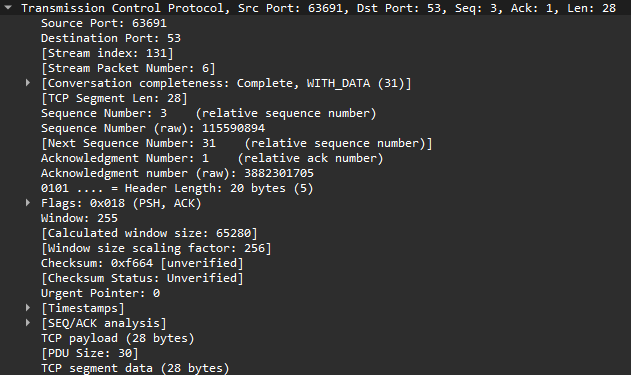
\includegraphics[width=\linewidth, height=0.4\textheight, keepaspectratio]{photos/2-8}
		\caption{TCP section inside the packet}
	\end{figure}
	
	And the TCP section inside the previous neighbouring packet can be observed as follows: 
	\begin{figure}[H]
		\centering
		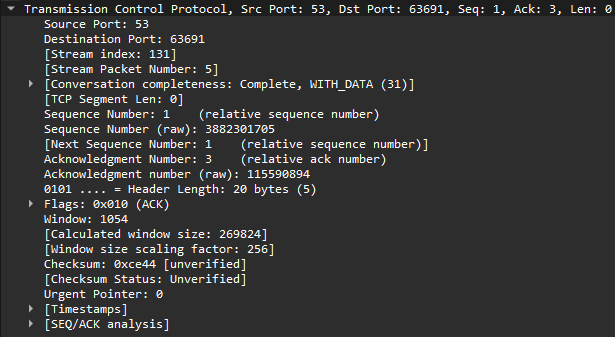
\includegraphics[width=\linewidth, height=0.4\textheight, keepaspectratio]{photos/2-8prev}
		\caption{TCP section inside the previous neighbouring packet}
	\end{figure}
	Comparing the Sequence number and Acknowledgement number of the two, it can be seen that sequence number of one packet is the acknowledgement number of the other, and vice versa. This is because TCP acknowledges the last byte received and indicates the next byte expected, enabling reliable two-way communication.
	
	The DNS server then acknowledges the incoming query, and sets the acknowledgement number to 31, meaning that it has successfully received the first 30 bytes from the client and expects the next byte starting at 31.
	\begin{figure}[H]
		\centering
		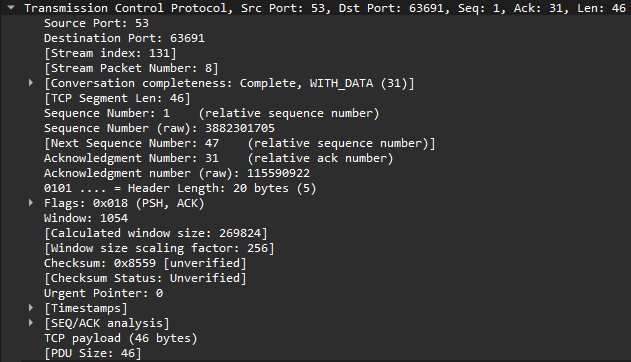
\includegraphics[width=\linewidth, height=0.4\textheight, keepaspectratio]{photos/2-9}
		\caption{DNS server standard query response}
	\end{figure}
	
	The following 4 packets after the response represent the four-way handshake to close the connection; in the output of wireshark, only three packets came up, however the flags set still resemble the process in the \textbf{abbreviated} form. The flags set were:
	\begin{enumerate}
		\item Server - [FIN, ACK]
		\item Client - [FIN, ACK]
		\item Server - [ACK]
	\end{enumerate}
	
	This is a faster alternative to the normal four-way handshake, which would have an additional Client - [ACK] after receiving from the server. 
	
	In CMD, the \texttt{nslookup} behaviour was set to the default state of using UDP for simple transmission by typing \texttt{set novc}.
	
	\vspace{1em}
	\hrule
	\vspace{0.5em}
	
	\section*{3. Objective 3}
	
	\textbf{Task Assignment:} The aim of this task was to compare the two protocols by means of graphs.
	
	\textbf{Solution:} \\ [1em]
	After using the same \texttt{dns.qry.name==www.vut.cz.localdomain} filter to display DNS conversations, one of the packets that used UDP as the transport protocol was selected. It was right clicked and \textbf{Follow > UDP Stream} was selected. The specified packets were exported. 
	
	The above process was then repeated for the TCP stream, and then the two were merged. 
	
	Following are the graphs comparing Packets for UDP and TCP 
	\begin{figure}[H]
		\centering
		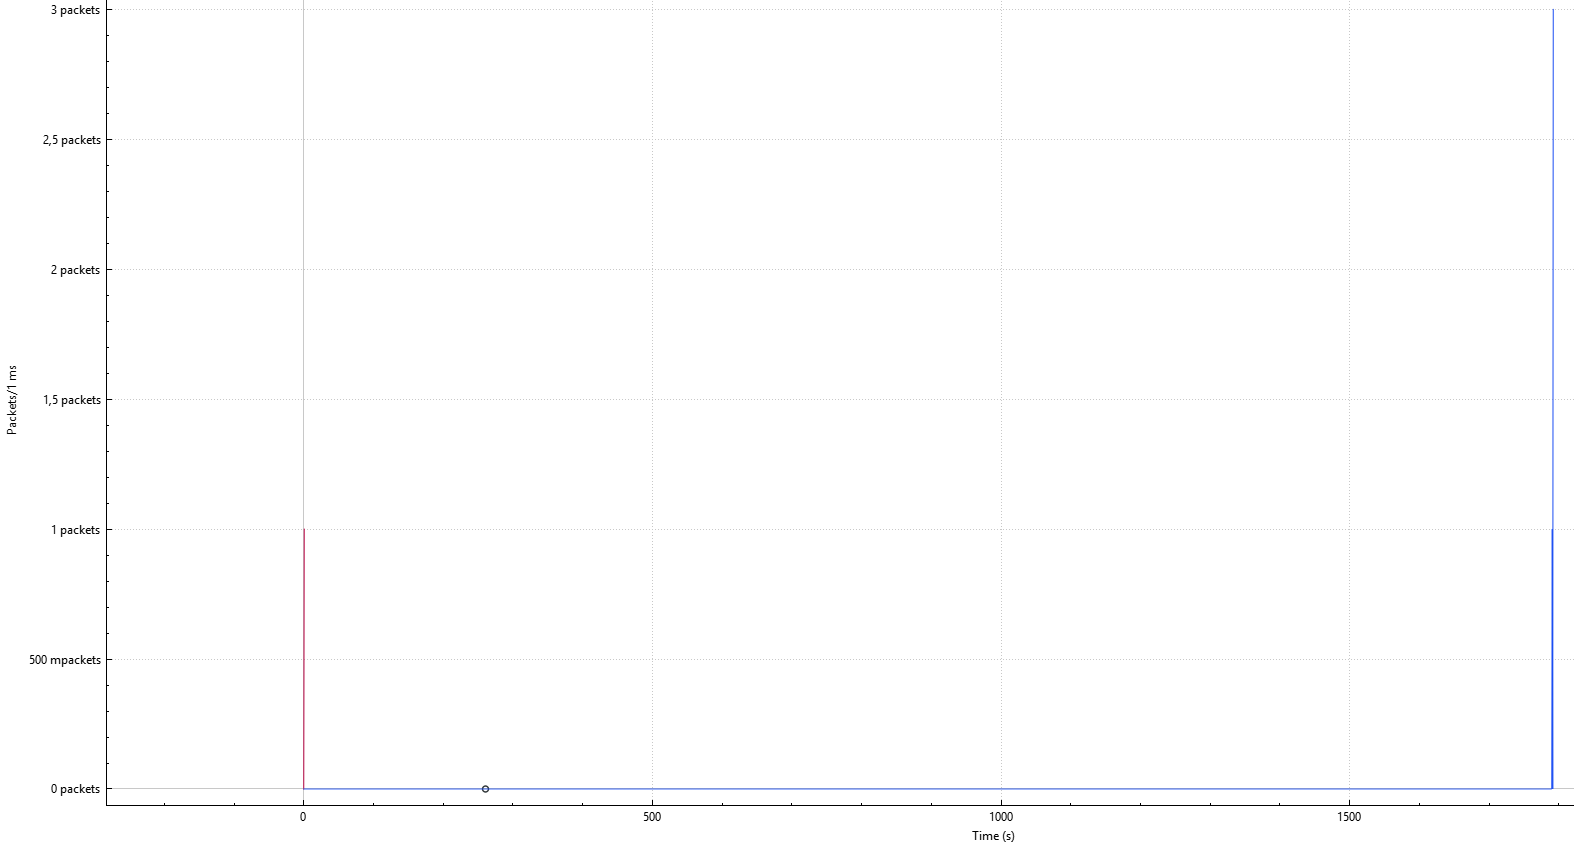
\includegraphics[width=\linewidth, height=0.4\textheight, keepaspectratio]{photos/3-6-packet}
		\caption{Packets sent during DNS transmissions using UDP(red) and TCP(blue)}
	\end{figure}
	
	In the Lab we were informed that there was a bug with Wireshark during the Lab, however, from the output, it can still be shown that more packets were used for the complete transmission in case of TCP (blue) than with UDP. The largest amount of packets per second for TCP was 3, and 1 for UDP.
	
	Following are the graphs comparing Bytes for UDP and TCP:
	\begin{figure}[H]
		\centering
		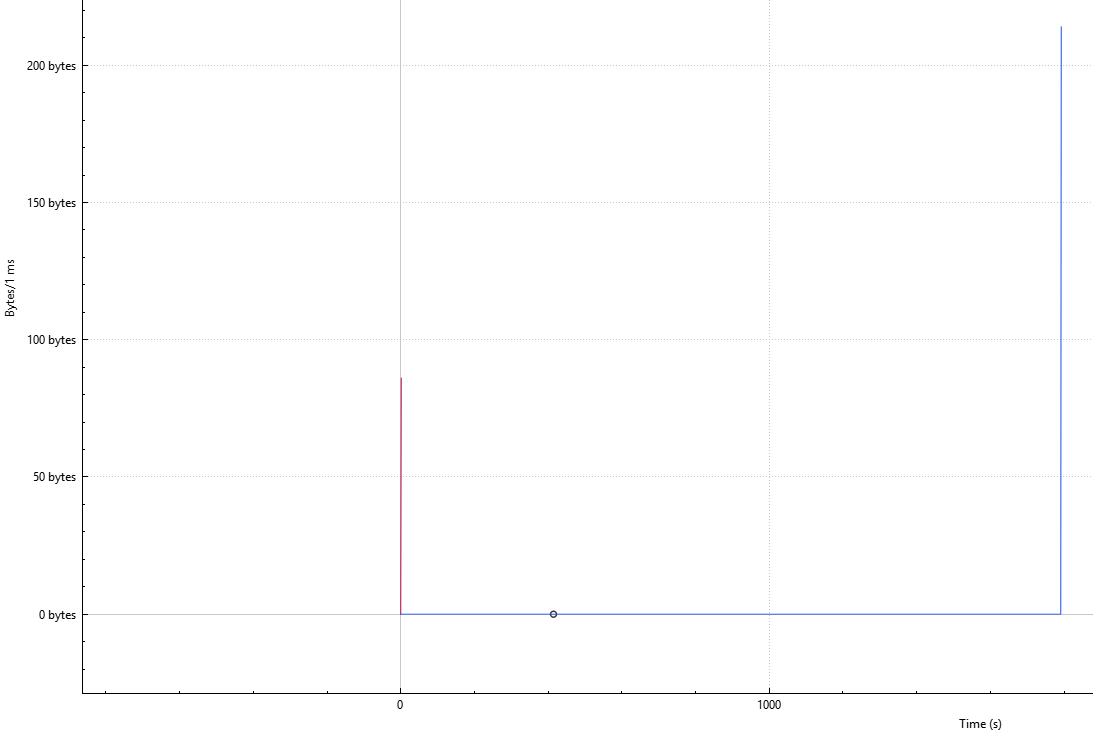
\includegraphics[width=\linewidth, height=0.4\textheight, keepaspectratio]{photos/3-6-bytes}
		\caption{Bytes sent during DNS transmission using UDP(red) and TCP(blue)}
	\end{figure}
	
	Once again, the output was bugged, however, it can still be seen that TCP transferred many more bytes per second; reaching ~210 at the peak, while UDP reached ~80. 
	
	Although Throughput of TCP was higher, in terms of time, UDP was faster in full query-response transfer. 
	
	\vspace{1em}
	\hrule
	\vspace{0.5em}
	
	\section*{4. Objective 4}
	
	\textbf{Task Assignment:} The aim of this task was to generate HTTP traffic in Wireshark.
	
	\textbf{Solution:}\\[1em]  
	To do this, the website \textit{http://www.neverssl.com} was visited, and after the content was loaded, the browser was closed and capturing in Wireshark was stopped. 
	
	After, any of the packets was right clicked and the TCP Stream was observed. A new pop up window with HTML structure opens as follows: 
	\begin{figure}[H]
		\centering
		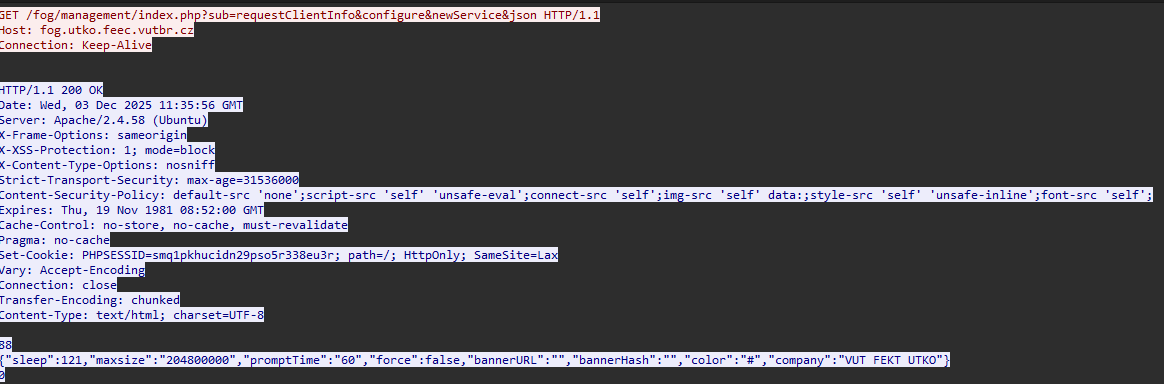
\includegraphics[width=\linewidth, height=0.4\textheight, keepaspectratio]{photos/4-2}
		\caption{Window with HTML structure}
	\end{figure}
	
	The TCP packets were then observed. There was some data loss during transmission, as indicated by the black highlighted rows in the output below.
	
	\begin{figure}[H]
		\centering
		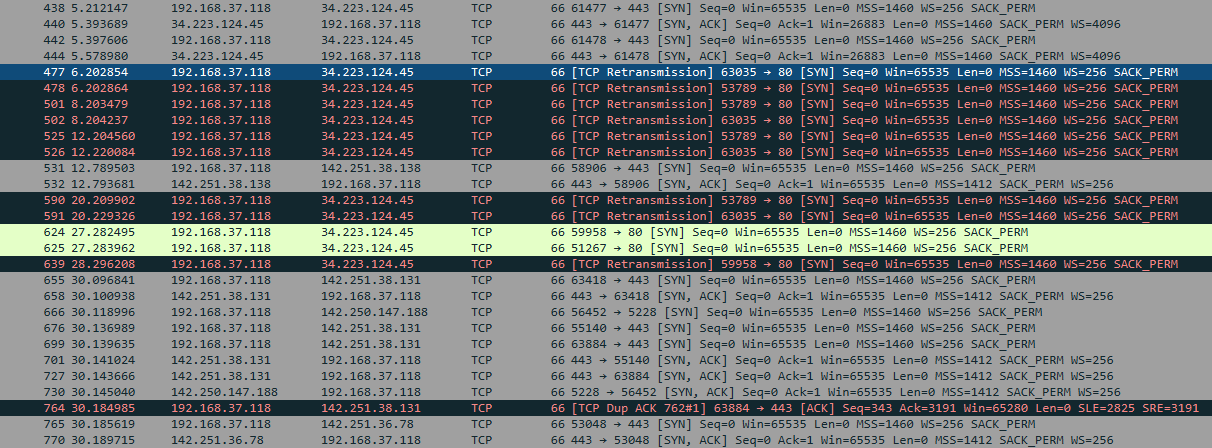
\includegraphics[width=\linewidth, height=0.4\textheight, keepaspectratio]{photos/4-4loss}
		\caption{Packet loss during the TCP transmission.}
	\end{figure}
	
	
	In my output, I did not have any message \textbf{TCP Previous segment not captured}. In the Lab it is asked why sequence number 1 is still expected from the client after such a message; this is because  TCP only acknowledges data that arrives in order, so even though a higher sequence number packet arrived, the client continues to request sequence number 1.
	
	In my output, i had messages \textbf{TCP Dup ACK} and \textbf{TCP Retransmission}. \textbf{TCP Dup ACK}means that the receiver sent the same acknowledgment number again, indicating that it is still expecting the same sequence number because some data has not been received. \textbf{TCP Retransmission} means that the sender retransmitted a data segment because it detected packet loss, usually after receiving duplicate acknowledgments (TCP Dup ACK).
	
	\vspace{1em}
	\hrule
	\vspace{0.5em}
	
	\section*{5. Objective 5}
	
	\textbf{Task Assignment:} The aim of this task was to create and configure the reference topology in Cisco Packet Tracer along with adding the new network to OSPF routing process.
	
	\textbf{Solution:}\\[1em]
	After adding the Server-PT device and adding it to the topology saved from previous labs, the topology is as follows:
	
	\begin{figure}[H]
		\centering
		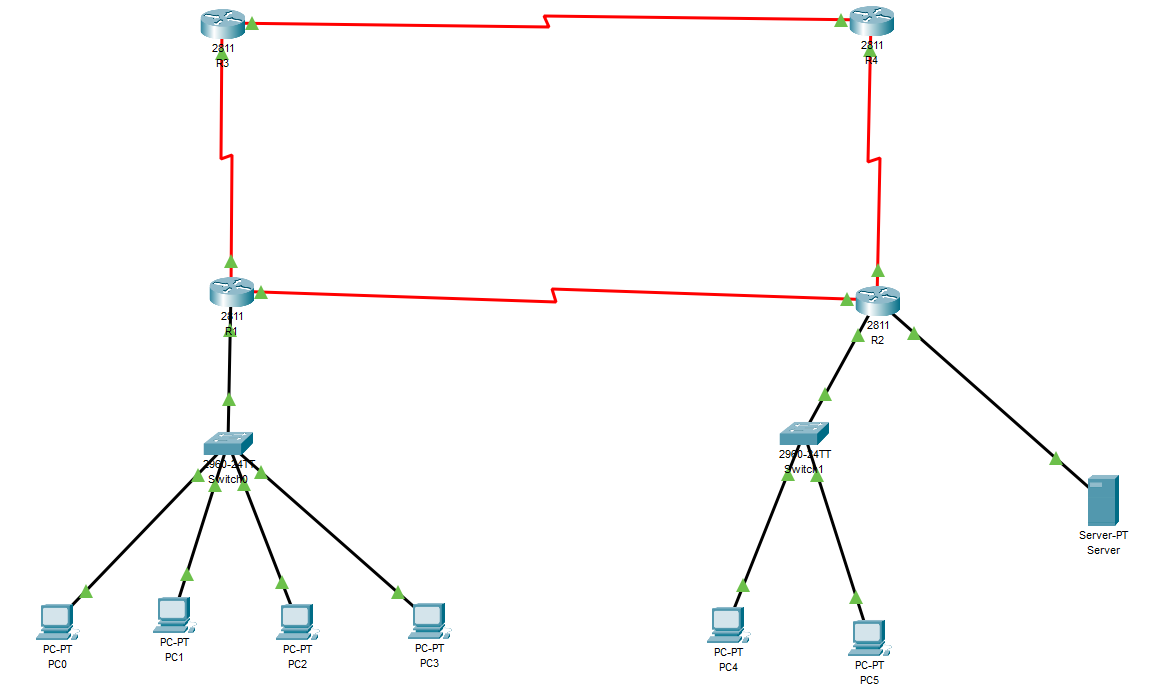
\includegraphics[width=\linewidth, height=0.4\textheight, keepaspectratio]{photos/5_topology}
		\caption{Current Topology in Cisco Packet Tracer.}
	\end{figure}
	
	After configuring the server and the router interface, R1's routing table was explored. The last entry of the table can be seen to be configured via RIP; this is because of the configuration from the last Lab. 
	
	\begin{figure}[H]
		\centering
		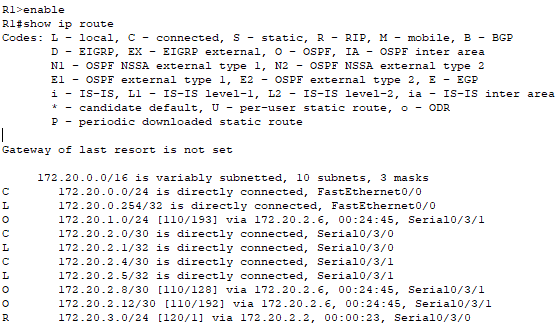
\includegraphics[width=\linewidth, height=0.4\textheight, keepaspectratio]{photos/obj5_4}
		\caption{R1 routing table with RIP path.}
	\end{figure}
	
	So to have routes learnt only via OSPF in the routing tables, \textit{172.20.3.0/24} subnet was added to the OSPF routing process. After this, R1's routing table was displayed again, and it can be seen that the RIP entry is now replaced by the OSPF entry. 
	
	\begin{figure}[H]
		\centering
		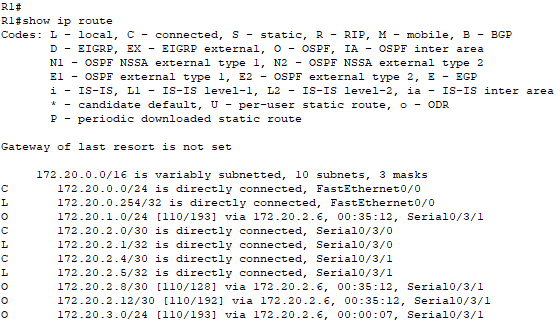
\includegraphics[width=\linewidth, height=0.4\textheight, keepaspectratio]{photos/obj5_6}
		\caption{R1 routing table with OSPF path.}
	\end{figure}
	
	The reachability of the server to R1's LAN was tested via the \texttt{ping} command. It was successful.
	
	\begin{figure}[H]
		\centering
		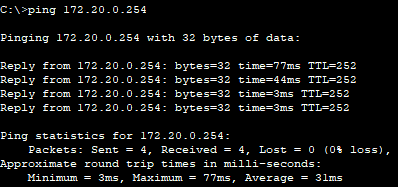
\includegraphics[width=\linewidth, height=0.4\textheight, keepaspectratio]{photos/obj5_8}
		\caption{ping command to test reachability of server to R1's LAN.}
	\end{figure}
	
	\vspace{1em}
	\hrule
	\vspace{0.5em}
	
	\section*{6. Objective 6}
	
	\textbf{Task Assignment:} The aim of this task was to start the DNS and HTTP services and create a web page on the server.
	
	\textbf{Solution:}\\[1em]
	By altering the configuration of services of the server, it was made as the DNS server and the web server for R1's LAN. 
	
	First, the HTTP was set up after editing the index.html file appropriately: 
	\begin{figure}[H]
		\centering
		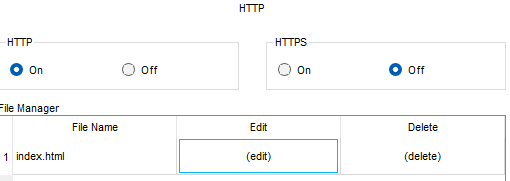
\includegraphics[width=\linewidth, height=0.2\textheight, keepaspectratio]{photos/obj6_3}
		\caption{HTTP service setup.}
	\end{figure}
	
	Then, the DNS service was configured as follows:
	\begin{figure}[H]
		\centering
		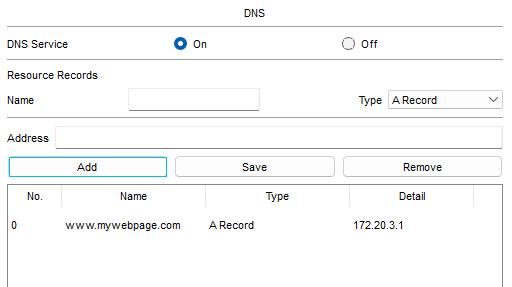
\includegraphics[width=\linewidth, height=0.2\textheight, keepaspectratio]{photos/obj6_4}
		\caption{DNS server configuration.}
	\end{figure}
	
	\vspace{1em}
	\hrule
	\vspace{0.5em}
	
	\section*{7. Objective 7}
	
	\textbf{Task Assignment:} The aim of this task was to configure the DNS server address on the PCs.
	
	\textbf{Solution:}\\[1em]
	So that the clients know which server to use for domain name translations, the DNS server address was set on the PCs of R1's LAN. The following is an example of one of the PCs. 
	\begin{figure}[H]
		\centering
		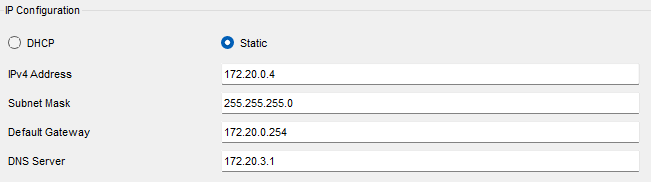
\includegraphics[width=\linewidth, height=0.4\textheight, keepaspectratio]{photos/obj7}
		\caption{DNS Server set up on PC of R1's LAN.}
	\end{figure}
	
	
	\vspace{1em}
	\hrule
	\vspace{5em}
	
	\section*{8. Objective 8}
	
	\textbf{Task Assignment:} The aim of this task was to access the server web page and analyse the traffic.
	
	\textbf{Solution:}\\[1em]
	For this objective, \textbf{Simulation} mode was activated, and the following protocols were selected for capturing:
	\begin{itemize}
		\item UDP
		\item TCP
		\item DNS
		\item HTTP
	\end{itemize}
	
	From a Pc from R1's LAN, \texttt{www.mywebpage.com} was entered into the Web Bowser. The webpage prints as follows: 
	\begin{figure}[H]
		\centering
		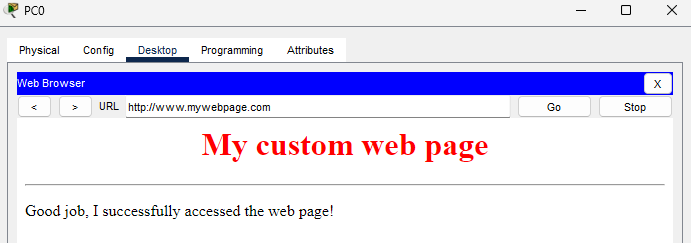
\includegraphics[width=\linewidth, height=0.3\textheight, keepaspectratio]{photos/obj8_webpage}
		\caption{Content of the webpage after formatting index.html.}
	\end{figure}
	
	This prompts a DNS datagram to appear in the event list. This is the content:
	\begin{figure}[H]
		\centering
		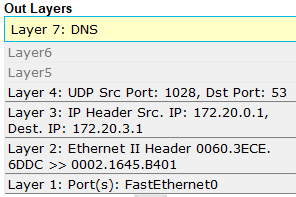
\includegraphics[width=\linewidth, height=0.3\textheight, keepaspectratio]{photos/obj8_4}
		\caption{Content of the DNS datagram.}
	\end{figure}
	It can be seen that the source port is 1028, and the Destination port is 52. The destination IP address is 172.20.3.1
	
	Capture then forward was then clicked until the datagram reaches the server. When it reaches, this is the outbound section: 
	
	\begin{figure}[H]
		\centering
		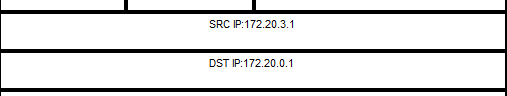
\includegraphics[width=\linewidth, height=0.1\textheight, keepaspectratio]{photos/obj8_6_1}
		\caption{Outbound section of the datagram reaching the server.}
	\end{figure}
	It can be seen that the Source and Destination ports, as happened in Wireshark, swap places with respect to the previous datagram.
	
	The DNS answer yields the following:
	\begin{figure}[H]
		\centering
		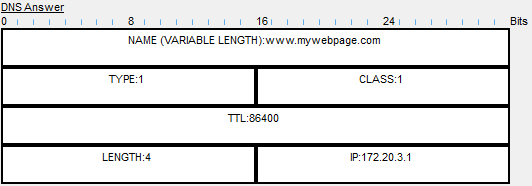
\includegraphics[width=\linewidth, height=0.2\textheight, keepaspectratio]{photos/obj8_6_2}
		\caption{DNS answer output.}
	\end{figure}
	The IP address the server is responding for the queried domain is 172.20.3.1.
	
	Capture then forward is then clicked again until the datagram reaches the PC. A new TCP segment is generated and the content is the following: 
	\begin{figure}[H]
		\centering
		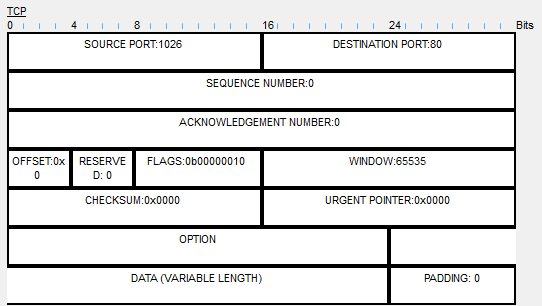
\includegraphics[width=\linewidth, height=0.3\textheight, keepaspectratio]{photos/obj8_7}
		\caption{Content of newly generated TCP segment.}
	\end{figure}
	From the content, the following can be seen: 
	\begin{itemize}
		\item Source port: 1026
		\item Destination port: 80
		\item Sequence number: 0
		\item Acknowledgment number: 0 
		\item Flags set: 1 (SYN)
	\end{itemize}
	
	Capture then forward is then clicked again until the datagram reaches the server. The content is the following:
	
	\begin{figure}[H]
		\centering
		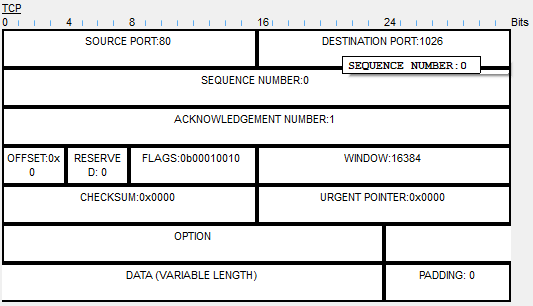
\includegraphics[width=\linewidth, height=0.3\textheight, keepaspectratio]{photos/obj8_8}
		\caption{Content of the datagram reaching the server.}
	\end{figure}
	From the content, the following can be seen: 
	\begin{itemize}
		\item Source port: 80
		\item Destination port: 1026
		\item Sequence number: 0
		\item Acknowledgment number: 1
		\item Flags set: 2 (SYN and ACK)
	\end{itemize}
	
	Capture then forward is then clicked again until the datagram reaches the PC once again. The content is the following:
	
	\begin{figure}[H]
		\centering
		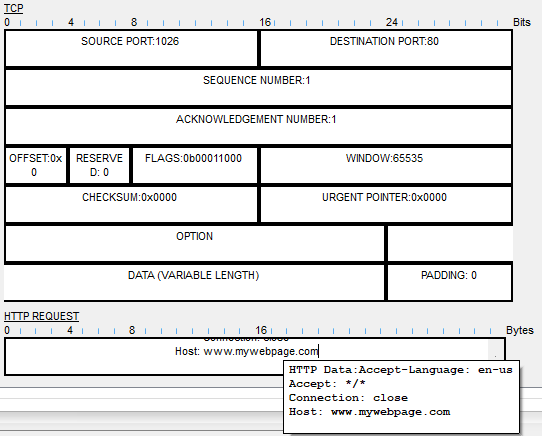
\includegraphics[width=\linewidth, height=0.4\textheight, keepaspectratio]{photos/obj8_9}
		\caption{Content of the datagram reaching the PC once again.}
	\end{figure}
	From the content, the following can be seen: 
	\begin{itemize}
		\item Source port: 1026
		\item Destination port: 80
		\item Sequence number: 1
		\item Acknowledgment number: 1
		\item Flags set: 2 (ACK and PSH)
		\item HTTP message transferred: REQUEST
	\end{itemize}
	
	This part represents the end of the three-way handshake, and HTTP messages are now transferred. 
	
	Capture then forward is then clicked again until the datagram reaches the server. Both the TCP segment finishing the three-way handshake and HTTP message are now transferred
	
	Once more, Capture then forward is clicked so that the HTTP message reaches the server. The contents are the following
	
	\begin{figure}[H]
		\centering
		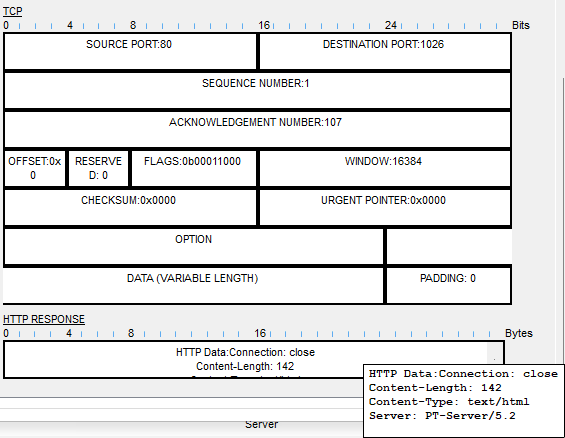
\includegraphics[width=\linewidth, height=0.4\textheight, keepaspectratio]{photos/obj8_11}
		\caption{Content of Outbound PDU details.}
	\end{figure}
	From the content, the following can be seen: 
	\begin{itemize}
		\item Source port: 80
		\item Destination port: 1026
		\item Sequence number: 1
		\item Acknowledgment number: 107
		\item Flags set: 2 (ACK and PSH)
		\item HTTP message transferred: RESPONSE
	\end{itemize}
	
	Capture then forward until HTTP message reaches the PC is performed, and a new TCP segment is generated. 
	
	\begin{figure}[H]
		\centering
		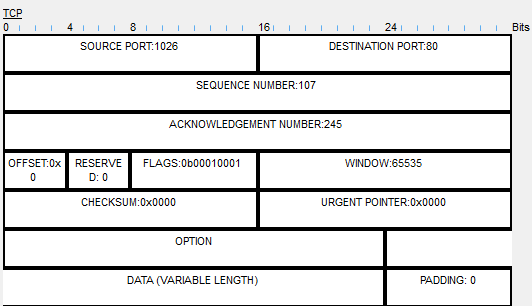
\includegraphics[width=\linewidth, height=0.4\textheight, keepaspectratio]{photos/obj8_12}
		\caption{Content of Outbound PDU details at the client.}
	\end{figure}
	From the content, the following can be seen: 
	\begin{itemize}
		\item Source port: 1026
		\item Destination port: 80
		\item Sequence number: 107 (previously 1)
		\item Acknowledgment number: 245 (previously 107)
		\item Flags set: 2 (FIN and ACK)
		\item HTTP message transferred: None as web page was successfully transferred.
	\end{itemize}
	
	Capture then forward is then performed until the segment reaches the server, and contents are the following:
	\begin{figure}[H]
		\centering
		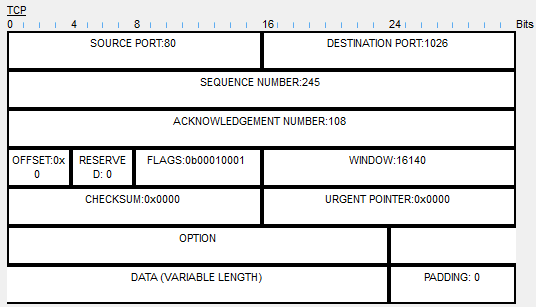
\includegraphics[width=\linewidth, height=0.4\textheight, keepaspectratio]{photos/obj8_13}
		\caption{Content of Outbound PDU details at the server.}
	\end{figure}
	From the content, the following can be seen: 
	\begin{itemize}
		\item Source port: 80
		\item Destination port: 1026
		\item Sequence number: 245
		\item Acknowledgment number: 108
		\item Flags set: 2 (FIN and ACK)
	\end{itemize}
	
	For the final time, capture then forward is performed until the segment reaches the client. The contents of the segment are the following: 
	\begin{figure}[H]
		\centering
		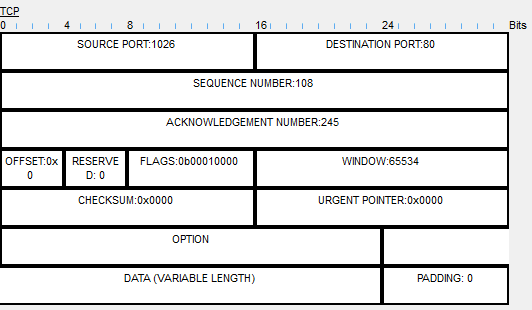
\includegraphics[width=\linewidth, height=0.25\textheight, keepaspectratio]{photos/obj8_14_1}
		\caption{Content of Outbound PDU details at the client.}
	\end{figure}
	From the content, the following can be seen: 
	\begin{itemize}
		\item Source port: 1026
		\item Destination port: 80
		\item Sequence number: 108
		\item Acknowledgment number: 245
		\item Flags set: 1 (ACK)
	\end{itemize}
	
	To verify that this is the last segment to close the connection, capture then forward is clicked until the segment reaches the server. As seen by the content, there is no new segment generated (the sequence number, acknowledgement number, and the flags are the same as before.)
	\begin{figure}[H]
		\centering
		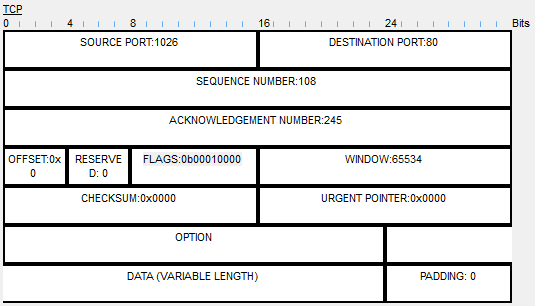
\includegraphics[width=\linewidth, height=0.3\textheight, keepaspectratio]{photos/obj8_14_2}
		\caption{Content of Outbound PDU details at the Server indicating no new changes.}
	\end{figure}
	
	\vspace{1em}
	\hrule
	\vspace{0.5em}
	
	\section*{9. Final Questions}
	
	
	\textbf{Question 1: What items does the UDP header contain?}\\
	The UDP header contains:
	\begin{itemize}
		\item \textbf{Source port:} identifies the sending application
		\item \textbf{Destination port:} identifies the receiving application
		\item \textbf{Length:} the length of the UDP header and data in bytes
		\item \textbf{Checksum:} used for error detection of the header and data
	\end{itemize}
	
	\textbf{Question 2: What happens when the packet is lost during UDP communication in comparison with TCP?}
	\begin{itemize}
		\item \textbf{UDP:} If a packet is lost, it is simply discarded, and no retransmission occurs.
		\item \textbf{TCP:} Detects lost packets using acknowledgments and retransmits them to ensure all data reaches the destination.
	\end{itemize}
	
	\textbf{Question 3: What precedes and follows the data exchange via TCP protocol?}
	\begin{itemize}
		\item \textbf{Precedes:} TCP connection establishment through the \textbf{three-way handshake}
		\item \textbf{Follows:} TCP connection termination through the \textbf{four-way handshake} or alternatively the abbreviated and faster \textbf{three-way handshake}. 
	\end{itemize}
	
	\textbf{Question 4: How is the TCP connection (virtual circuit) establishment called?}\\
	
	TCP connection establishment is called the \textbf{three-way handshake}, which involves SYN, SYN+ACK, and ACK messages.
	
	\textbf{Question 5: What groups of ports do the servers use for common services?}
	\begin{itemize}
		\item \textbf{Well-known ports (0–1023):} These ports are used by servers providing common services. Clients commonly use them as destination ports when initiating communication.
		\item \textbf{Registered ports (1024–49151):} These ports are used by both clients and servers. For client purposes, some of this range may be reserved by the operating system. For server purposes, they must be registered by IANA.
		\item \textbf{Dynamic/Private ports (49152–65535):} These ports are dynamically assigned to clients when initiating communication.
	\end{itemize}
	

	
	\vspace{1em}
	\hrule
	\vspace{0.5em}
	
\end{document}
